%
% qclsip: The Quantum Cascade Laser Stock Image Project.
%
% Copyright (c) 2019, Computational Photonics Group, Technical University of
% Munich.
%
% Mathematical model of a QCL (Schrödinger-Poisson, Ensemble Monte Carlo,
% Maxwell's equation, Lindblad equation).
% Created by Michael Riesch <michael.riesch@tum.de> (2019)
%
% This program is free software; you can redistribute it and/or modify
% it under the terms of the GNU General Public License as published by
% the Free Software Foundation; either version 3 of the License, or
% (at your option) any later version.
%
% This program is distributed in the hope that it will be useful,
% but WITHOUT ANY WARRANTY; without even the implied warranty of
% MERCHANTABILITY or FITNESS FOR A PARTICULAR PURPOSE.  See the
% GNU General Public License for more details.
%
% You should have received a copy of the GNU General Public License
% along with this program; if not, write to the Free Software Foundation,
% Inc., 51 Franklin Street, Fifth Floor, Boston, MA 02110-1301  USA
\documentclass[tikz]{standalone}

\usepackage[utf8]{inputenc}
\usepackage[T1]{fontenc}
\usepackage{tikz}
\usetikzlibrary{calc}

% set colors
\usepackage{xcolor}
\definecolor{sipblue}{RGB}{0,101,189} % Pantone 300
\definecolor{sipdarkblue}{RGB}{0,82,147} % Pantone 301
\definecolor{siplightblue}{RGB}{152,198,234} % Pantone 283
\definecolor{sipmedblue}{RGB}{100,160,200} % Pantone 542
\definecolor{sipivory}{RGB}{218,215,203} % Pantone 7527
\definecolor{sipgreen}{RGB}{162,173,0} % Pantone 383
\definecolor{siporange}{RGB}{227,114,34} % Pantone 158
\definecolor{sipgray}{gray}{0.6} % Gray 60%

% set font
\usepackage{helvet}
\renewcommand{\familydefault}{\sfdefault}

\begin{document}
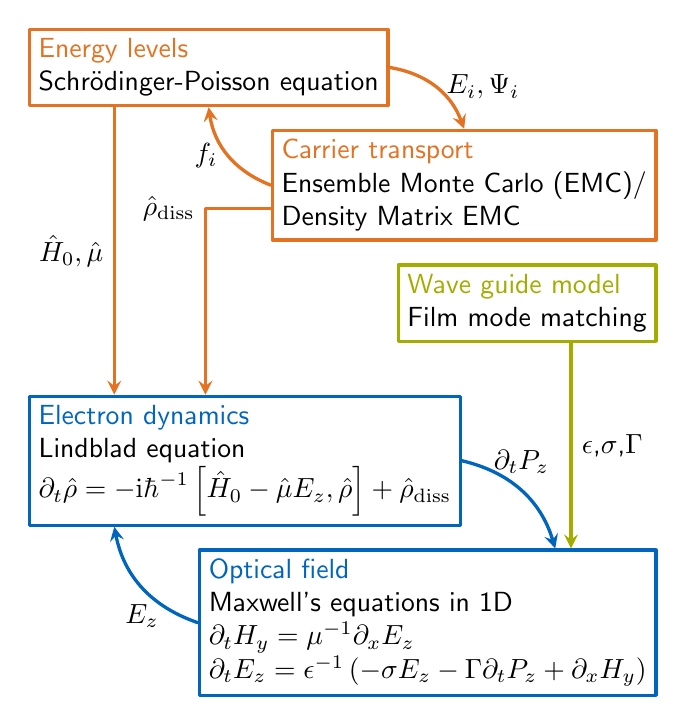
\begin{tikzpicture}
  \tikzstyle{myline}=[very thick, line cap=round,line join=round];
  \tikzstyle{mytext}=[draw, text=black, align=left];
  \tikzstyle{myconn}=[myline, ->, >=stealth];
  %
  % static part
  \node[mytext, myline, draw=siporange, anchor=north west] (sp) at (0, 7) {
    \textcolor{siporange}{Energy levels}\\Schrödinger-Poisson equation};
  %
  \node[mytext, myline, draw=siporange, anchor=east] (mc) at (8, 5) {
    \textcolor{siporange}{Carrier transport}\\Ensemble Monte Carlo (EMC)/\\
    Density Matrix EMC};
  %
  % wave guide part
  \node[mytext, myline, draw=sipgreen, anchor=east] (wg) at (8, 3.5) {
    \textcolor{sipgreen}{Wave guide model}\\Film mode matching};
  %
  % dynamic part
  \node[mytext, myline, draw=sipblue, anchor=west] (lb) at (0, 1.5) {
    \textcolor{sipblue}{Electron dynamics}\\Lindblad equation\\
    $\partial_t \hat{\rho} = -\mathrm{i}\hbar^{-1} \left[ \hat{H}_0 -
      \hat \mu E_z, \hat{\rho} \right] + \hat{\rho}_{\mathrm{diss}}$};
  %
  \node[mytext, myline, draw=sipblue, anchor=south east] (mw) at (8, -1.5) {
    \textcolor{sipblue}{Optical field}\\Maxwell's equations in 1D\\
    $\partial_t H_y = \mu^{-1} \partial_x E_z$\\
    $\partial_t E_z = \epsilon^{-1} \left( -\sigma E_z - \Gamma \partial_t P_z +
    \partial_x H_y \right)$};
  %
  % connections
  \draw[myconn, draw=siporange] (sp.east) to[bend left] node[midway, right] {
    $E_i, \Psi_i$} (mc.north);
  %
  \draw[myconn, draw=siporange] (mc.west) to[bend left] node[midway, left] {
    $f_i$} (sp.south);
  %
  \draw[myconn, draw=siporange] ($(sp.south west) + (1.1, 0)$)
  -- node[midway, left] {$\hat H_0, \hat \mu$}
  ($(lb.north west) + (1.1, 0)$);
  %
  \draw[myconn, draw=siporange] ($(mc.west) - (0, 0.3)$)
  -| node[midway, left] {$\hat{\rho}_{\mathrm{diss}}$}
  ($(lb.north) - (0.5, 0)$);
  %
  \draw[myconn, draw=sipblue] (mw.west)
  to[bend left] node[midway, below, outer sep=3pt] {$E_z$}
  ($(lb.south west) + (1.1, 0)$);
  %
  \draw[myconn, draw=sipblue] (lb.east)
  to[bend left] node[midway, above, outer sep=3pt] {$\partial_t P_z$
    %    $= N \mathrm{Tr}\left\{\hat \mu \partial_t \hat \rho\right\}$
  }
  ($(mw.north east) - (1.3, 0)$);
  %
  \draw[myconn, draw=sipgreen] ($(wg.south east) - (1.1, 0)$)
  -- node[midway, right] {$\epsilon$,$\sigma$,$\Gamma$}
  ($(mw.north east) - (1.1, 0)$);
\end{tikzpicture}
\end{document}
